\documentclass[10pt,twocolumn,letterpaper]{article}

\usepackage{cvpr}
\usepackage{times}
\usepackage{epsfig}
\usepackage{graphicx}
\usepackage{amsmath}
\usepackage{amssymb}
\graphicspath{{Images/}{../FinalPresentation/Images/}}

% Include other packages here, before hyperref.

% If you comment hyperref and then uncomment it, you should delete
% egpaper.aux before re-running latex.  (Or just hit 'q' on the first latex
% run, let it finish, and you should be clear).
\usepackage[breaklinks=true,bookmarks=false]{hyperref}

\cvprfinalcopy % *** Uncomment this line for the final submission

\def\cvprPaperID{****} % *** Enter the CVPR Paper ID here
\def\httilde{\mbox{\tt\raisebox{-.5ex}{\symbol{126}}}}

% Pages are numbered in submission mode, and unnumbered in camera-ready
%\ifcvprfinal\pagestyle{empty}\fi
\setcounter{page}{1}
\begin{document}

%%%%%%%%% TITLE
\title{Fooling Pneumonia Classification with Normalizing Flows}

\author{Luis Guzman\\
University of Oregon\\
{\tt\small lguzman@uoregon.edu}
% For a paper whose authors are all at the same institution,
% omit the following lines up until the closing ``}''.
% Additional authors and addresses can be added with ``\and'',
% just like the second author.
% To save space, use either the email address or home page, not both
\and
Steven Walton\\
University of Oregon\\
{\tt\small swalton2@uoregon.edu}
}

\maketitle
%\thispagestyle{empty}

%%%%%%%%% ABSTRACT
\begin{abstract} 
    The goal of this project was to learn about how to implement
    Normalizing Flows and demonstrate this by generating a flow that is able to
    generate x-ray images that can trick a pneumonia classifier.  In this work
    we detail our Normalizing Flow network, based off of GLOW, that is able to
    fool several deep neural network classifiers over 96\% of the time.  This
    work shows that normalizing flows are able to generate quality images,
    meaning that the learn the distribution with reasonable accuracy and that we
    could replicate a state of the art normalizing flow implementation. 
\end{abstract}

%%%%%%%%% BODY TEXT
\section{Introduction}
Normalizing Flows are a powerful type of generative model, similar to Generative
Adversarial Networks (GANs) and Variational Autoencoders (VAEs). While GANs and
VAEs implicitly learn the distribution of a dataset, Normalizing Flows
explicitly learn the distribution. In this project we attempt to learn the
explicit representation of pneumonia cases in x-rays. To test the effectiveness
of this learning we train classical classifiers on this dataset and have them
classify our generated images.

\subsection{Related Work}
Generative models are a popular framework for machine learning because they are
able to generate new instances of a dataset. For example, a model that has
trained on what cats look like is able to generate a new cat, an example of
which can be found with the popular website
ThisCatDoesNotExist.com~\cite{tcdne}. GANs have become popular types of
generative models because they are able to produce high quality and realistic
images. Normalizing flows have gained attention because of their ability to
learn the exact dataset and get the logliklihood while still producing sharp
images. 

NICE~\cite{nice}, Non-Linear Independent Component Estimation,  was a
foundational work on normalizing flows demonstrating that with a simple flow
model a high-dimensional dataset could be learned. NICE uses a simple additive
coupling layer, using a linear function. They simplified the inverse function by
using a function that has a unit Jacobian determinant. This makes the inverse
trivial to compute, since the determinant is 1. While NICE isn't competitive
with GANs from the same time, it did demonstrate that normalizing flows can be
easily trained and constructed.

RealNVP~\cite{realnvp}, which stands for real-valued non-volume preserving, was
a follow-up paper to NICE that improved on the results. 

\subsection{Normalizing Flows}

\section{Details of Approach}

\section{Results}
In this section incrementally presents the results we obtained while working on the current project.
\subsection{NICE results}
As mentioned previously, we first implemented the NICE~\cite{nice} model. Figure~\ref{fig:forward_pass} showcases the the transformation of an input image after it has passed through the model. Given that NF models are completely reversible, if the transformed image shown in Figure~\ref{fig:transformed} is put through the backward pass of the model the original image (Figure \ref{fig:original}) is obtained.  Conversely, Figure \ref{fig:backward_pass} shows how images are generated by sampling a random vector from the prior distribution (multi-variate Gaussian in our experiments) and putting it through the backward pass of the NF model.
    \begin{figure}[htbp!]
     \centering
     \begin{subfigure}[b]{0.45\textwidth}
         \centering
         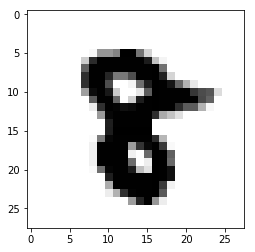
\includegraphics[width=0.5\textwidth]{input.png}
         \caption{Input image}
         \label{fig:original}
     \end{subfigure} 
     \hfill
     \begin{subfigure}[b]{0.45\textwidth}
         \centering
         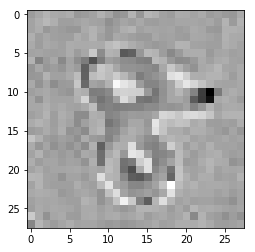
\includegraphics[width=0.5\textwidth]{transformed.png}
         \caption{Transformed}
         \label{fig:transformed}
     \end{subfigure}
     \hfill
     \caption{Transformation of an input image via forward pass.}
     \label{fig:forward_pass}
\end{figure}

    \begin{figure}[htbp!]
     \centering
     \begin{subfigure}[b]{0.45\textwidth}
         \centering
         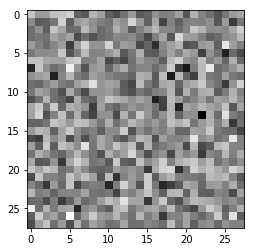
\includegraphics[width=0.5\textwidth]{sample.png}
         \caption{Sample from prior}
     \end{subfigure} 
     \hfill
     \begin{subfigure}[b]{0.45\textwidth}
         \centering
         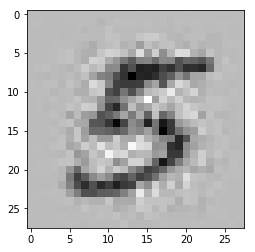
\includegraphics[width=0.5\textwidth]{generated.png}
         \caption{Generated image}
     \end{subfigure}
     \hfill
     \caption{Image generation with backward pass}
     \label{fig:backward_pass}
\end{figure}

The generation results after training two equivalent NICE models on both the MNIST and FashionMNIST data sets are shown in Figure~\ref{fig:nice_results}. The top image (\ref{fig:random_samples}) shows the vectors randomly sampled from the prior distribution, while the middle (\ref{fig:mnist_results}) and bottom (\ref{fig:fashion_results}) show the generated images created by transforming such sampled vectors by the MNIST and FashionMNIST models, respectively.

\begin{figure}[htbp!]
     \centering
     \begin{subfigure}[b]{0.3\textwidth}
         \centering
         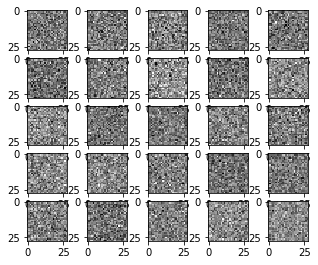
\includegraphics[width=\textwidth]{prior2.png}
         \caption{Sampled vectors}
         \label{fig:random_samples}
     \end{subfigure} 
     \hfill
     \begin{subfigure}[b]{0.3\textwidth}
         \centering
         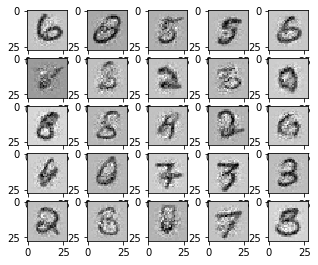
\includegraphics[width=\textwidth]{mnist2.png}
         \caption{MNIST}
         \label{fig:mnist_results}
     \end{subfigure}
     \hfill
     \begin{subfigure}[b]{0.3\textwidth}
         \centering
         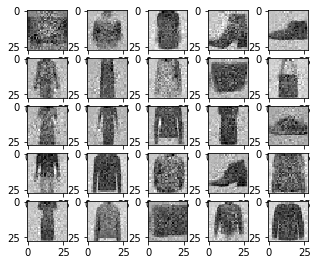
\includegraphics[width=\textwidth]{fashion2.png}
         \caption{FashionMNIST}
         \label{fig:fashion_results}
     \end{subfigure}
     \caption{NICE image generation results.}
     \label{fig:nice_results}
\end{figure}

It is apparent that the images generated by the NICE models are not great. We attribute this to the fact that the NICE normalizing flow is a very shallow one (using only 4 stacked layers), it only uses additive coupling layers, and relies on manually reversing the roles of the features partition subsets to ensure that all dimensions are transformed. All of these characteristics limit the models ability to learn complex distributions. 

\subsection{GLOW results}

Next we implemented the GLOW~\cite{glow} model. We purposely skipped implementing RealNVP~\cite{realnvp} because all of its innovations with respect to NICE, specifically the use of Affine coupling layers and the Multi-scale framework, are also used in GLOW. We trained our GLOW implementation on both CIFAR10 and the CelebA data sets. Here we present some results from the later one, which we find to be more relevant.

Figure~\ref{fig:glow_results} shows some image generation results for vectors sampled at different temperatures $\tau$. The images at the top row are sampled at $\tau = 0$ and thus all of the generated images are the same. The images at the bottom row are sampled at $\tau = 1$. It can be observed that as $\tau$ increases the presence of artifacts becomes more prevalent in the generated images. We found, empirically, that a $\tau$ value between $[0.2-0.6]$ yielded the best results, qualitatively.
    \begin{figure}
        \centering
        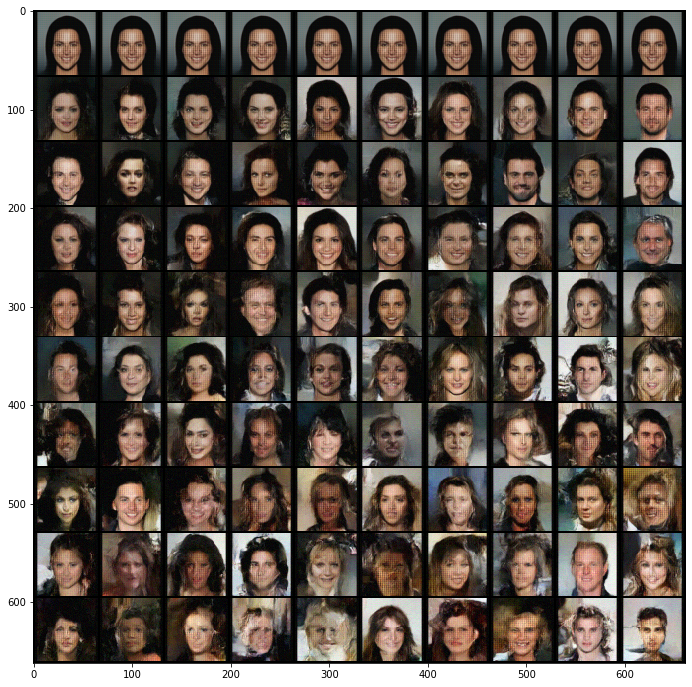
\includegraphics[width=0.5\textwidth]{celeb_multiple_stds2.png}
        \caption{GLOW generation results}
        \label{fig:glow_results}
    \end{figure}

We trained 2 distinct GLOW models with images with dimensionality of 64, and 128, respectively. Figure \ref{fig:glow_results2} shows some examples of the images generated by our models. While these results still do not achieve the same level of quality than the ones presented it the GLOW paper, we think they are sufficiently good given the computing resources available to us at the time. In particular, we were unable to train models that were as deep as the ones used in the original paper and also we could not train at 512 x 512 dimensionality.    

    \begin{figure}[htbp!]
     \centering
     \begin{subfigure}[b]{0.3\textwidth}
         \centering
         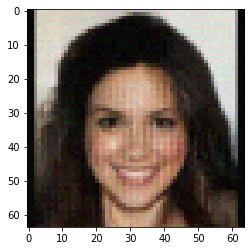
\includegraphics[width=\textwidth]{celeb_sample2.png}
         %\caption{MNIST}
     \end{subfigure}
     \hfill
     \begin{subfigure}[b]{0.3\textwidth}
         \centering
         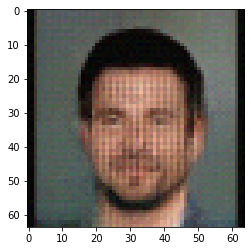
\includegraphics[width=\textwidth]{celeb_sample3.png}
         \caption{64 x 64 images}
     \end{subfigure}
     \hfill
     \begin{subfigure}[b]{0.3\textwidth}
         \centering
         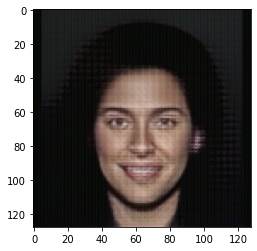
\includegraphics[width=\textwidth]{celeb_sample5.png}
         %\caption{MNIST}
     \end{subfigure}
     \hfill
     \begin{subfigure}[b]{0.3\textwidth}
         \centering
         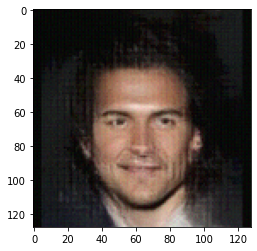
\includegraphics[width=\textwidth]{celeb_sample6.png}
         \caption{128 x 128 images}
     \end{subfigure}
     \hfill

     \caption{Images generated with GLOW}
     \label{fig:glow_results2}
\end{figure}

\subsection{X-ray data}

As discussed previously, our ultimate goal is to train a NF model that is able to fool a classifier. Thus, we first trained three distinct CNN-based (VGG19, Alexnet, Resnet50) classifiers on the Chest X-ray data set \footnote{https://www.kaggle.com/paultimothymooney/chest-xray-pneumonia}. Figure~\ref{fig:x_rays} shows some examples from both normal (\ref{fig:normal}) and pneumonia (\ref{fig:pneumonia}) images. Figure \ref{fig:classifiers_performance} shows the accuracy on the validation set for each of the classifiers. It can be observed that all of them achieve a fairly high validation accuracy of $\sim 90\%$.
    \begin{figure}
        \centering
        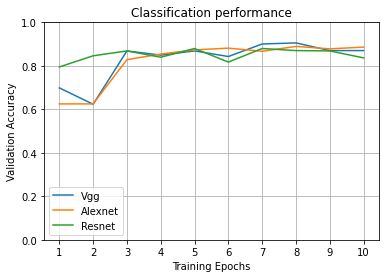
\includegraphics[width=.5\textwidth]{classification_performance.png}
        \caption{Classifiers validation performance.}
        \label{fig:classifiers_performance}
    \end{figure}
\begin{figure}[htbp!]
     \centering
     \begin{subfigure}[b]{0.3\textwidth}
         \centering
         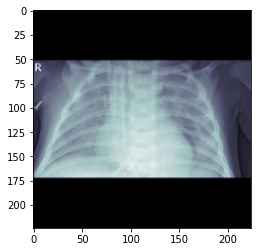
\includegraphics[width=\textwidth]{xray_normal1.png}
         %\caption{Sampled vectors}
     \end{subfigure} 
     \hfill
     \begin{subfigure}[b]{0.3\textwidth}
         \centering
         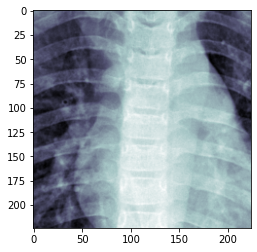
\includegraphics[width=\textwidth]{xray_normal3.png}
         \caption{Normal examples.}
         \label{fig:normal}
     \end{subfigure}
     \hfill
     \begin{subfigure}[b]{0.3\textwidth}
         \centering
         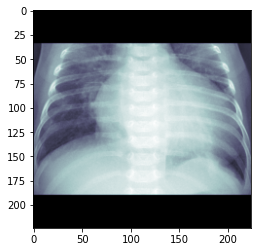
\includegraphics[width=\textwidth]{xray_pneumonia1.png}
         %\caption{Sampled vectors}
     \end{subfigure} 
     \hfill
     \begin{subfigure}[b]{0.3\textwidth}
         \centering
         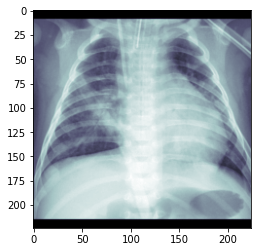
\includegraphics[width=\textwidth]{xray_pneumonia2.png}
         \caption{Pneumonia examples}
         \label{fig:pneumonia}
     \end{subfigure}
     \hfill
     \caption{Samples from X-ray dataset}
     \label{fig:x_rays}
\end{figure}

We then trained a 5-level GLOW model with a depth of 24 for each level using the Pneumonia-labeled images ($\sim 4K$) from the dataset. Given that our ultimate goal is to fool the classifiers, we trained on 224 x 224 images which are the expected input dimensions for our classifier models. 

Figure \ref{fig:xray_results} shows some examples the images generated by our model. It is apparent that our results would not be able to fool a human M.D. While they do share some resemblance with the images from the data set, they lack definition and other important features that would allow them to pass for real X-rays.

We believe there are two main reasons for our generation results poor performance: (1) we do not have sufficient data available for our model to satisfactory approximate the unknown distribution. There's only around 4K pneumonia images available, while we are using vectors with $> 50k$ features. And (2) given our computation resources constraints, we had to use a very small batch size of 5 and could not train a sufficiently deep model.

\begin{figure}[htbp!]
     \centering
     \begin{subfigure}[b]{0.3\textwidth}
         \centering
         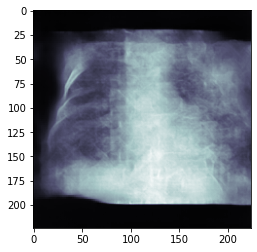
\includegraphics[width=\textwidth]{xray_sample2.png}
         %\caption{MNIST}
     \end{subfigure}
     \hfill
     \begin{subfigure}[b]{0.3\textwidth}
         \centering
         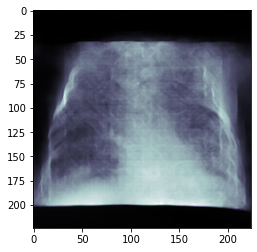
\includegraphics[width=\textwidth]{xray_sample3.png}
         %\caption{FashionMNIST}
     \end{subfigure}
     \hfill
     \begin{subfigure}[b]{0.3\textwidth}
         \centering
         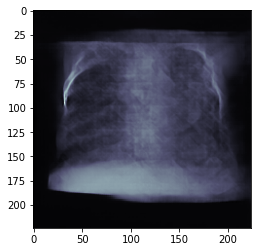
\includegraphics[width=\textwidth]{xray_sample5.png}
         %\caption{MNIST}
     \end{subfigure}
     \hfill
     \begin{subfigure}[b]{0.3\textwidth}
         \centering
         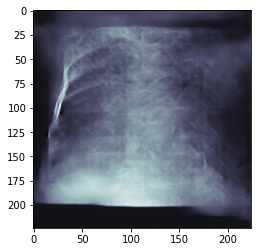
\includegraphics[width=\textwidth]{xray_sample6.png}
         %\caption{FashionMNIST}
     \end{subfigure}
     \caption{Generated x-ray images}
     \label{fig:xray_results}
\end{figure}

Our goal, however, is not to fool a human critic, but our classifier models trained on the data set. So, we generated some images using our model sampled at $\tau = [0.65, 0.7, 0.75, 0.8, 0.85, 0.9]$ (Figure \ref{fig:pneumonia_test_samples}) and put them through our classifiers. We found that both the Alexnet and VGG based classifiers were consistently fooled by the generated images achieving a $96\%$ fooling success rate. However, we obtained a $0\%$ fooling rate for the Resnet-based classifier. 

We believe the high-fooling rate achieved by our generated images is mainly caused by a bias of the Alexnet and VGG classification models towards predicting the Pneumonia class. This bias is probably caused by the fact that the data set is imbalanced toward such class. Nonetheless, the validation set used to report the classifiers performance does not display such a marked imbalance. Thus, we consider our reported classifier performance results to be valid.  

    \begin{figure}[!htbp]
        \centering
        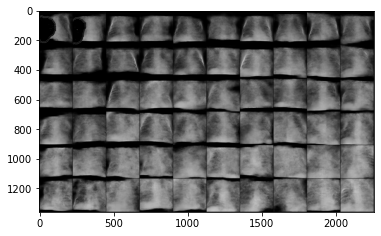
\includegraphics[width=.5\textwidth]{xray_test_example.png}
        \caption{Pneumonia generated images used for testing.}
        \label{fig:pneumonia_test_samples}
    \end{figure}

Finally, we tested our models ability to fool the classifiers to produce the Normal class instead. We trained an equivalent GLOW model with the Normal-labeled images from the dataset ($\sim 3K$) and generated images sampled at $\tau = [0.8, 0.85, 0.9, 0.95]$ (Figure \ref{fig:normal_test_samples}). Using these images we achieved fooling success rates of $65\%$, $32.5\%$, and $42.5\%$ for the Alexnet, VGG, and Resnet classifiers, respectively. Thus confirming our assumptions of our classifiers biases.

    \begin{figure}[!htbp]
        \centering
        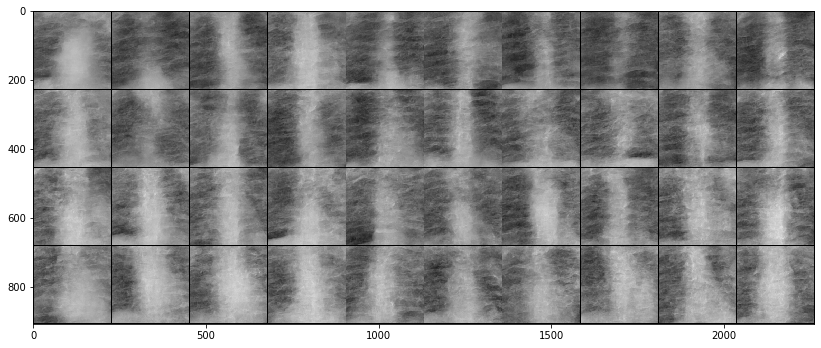
\includegraphics[width=.5\textwidth]{normal_generated.png}
        \caption{Normal generated images used for testing.}
        \label{fig:normal_test_samples}
    \end{figure}


\section{Discussion and Conclusions}

\section{Statement of Individual Contributions}
Both participants of this project contributed equally. The beginning of the
project focused on research within the area of normalizing flows. Steven
presented the idea of working with normalizing flows after reading Lilian Weng's
blog~\cite{weng2018flow} and Luis suggested using them to generate fake Covid
data, which we settled on just pneumonia cases since we found clearer and larger
datasets for that. 

The first step of the project was to build our background understanding. So we
each read NICE, RealNVP, GLOW, and FFJORD. We split these up so that each person
dug deeper on an individual paper. We then set up a Zoom meeting where we each
made slides and presented a deeper understanding of the papers to one another. 
Luis presented on NICE and FFJORD while Steven presented on RealNVP and GLOW. 

The next step both Luis and Steven independently tried to replicate the NICE
paper. When either one was confused on one section they consulted with the
other. Both ended up producing a network that was able to produce similar images
to NICE. The process was then repeated for advancing to GLOW. For the results we
used LUIS's network because his results turned out better than Steven's. We then
retrained AlexNet, ResNet, and VGG to perform a binary classification on the
pneumonia dataset. 


{\small
\bibliographystyle{ieee_fullname}
\bibliography{egbib}
}

\end{document}
